\documentclass[a4paper, 14pt]{extarticle}
\usepackage[settings]{markdown}
\usepackage{minted}

% Поля
%--------------------------------------
\usepackage{geometry}
\geometry{a4paper,tmargin=2cm,bmargin=2cm,lmargin=3cm,rmargin=1cm}
%--------------------------------------


%Russian-specific packages
%--------------------------------------
\usepackage[T2A]{fontenc}
\usepackage[utf8]{inputenc} 
\usepackage[english, main=russian]{babel}
%--------------------------------------

\usepackage{textcomp}

% Красная строка
%--------------------------------------
\usepackage{indentfirst}               
%--------------------------------------             


%Graphics
%--------------------------------------
\usepackage{graphicx}
\graphicspath{ {./images/} }
\usepackage{wrapfig}
%--------------------------------------

% Полуторный интервал
%--------------------------------------
\linespread{1.3}                    
%--------------------------------------

%Выравнивание и переносы
%--------------------------------------
% Избавляемся от переполнений
\sloppy
% Запрещаем разрыв страницы после первой строки абзаца
\clubpenalty=10000
% Запрещаем разрыв страницы после последней строки абзаца
\widowpenalty=10000
%--------------------------------------

%Списки
\usepackage{enumitem}

%Подписи
\usepackage{caption} 

%Гиперссылки
\usepackage{hyperref}

\hypersetup {
	unicode=true
}

%Рисунки
%--------------------------------------
\DeclareCaptionLabelSeparator*{emdash}{~--- }
\captionsetup[figure]{labelsep=emdash,font=onehalfspacing,position=bottom}
%--------------------------------------

\usepackage{tempora}
\usepackage{amsmath}
\usepackage{color}
\usepackage{listings}
\lstset{
  belowcaptionskip=1\baselineskip,
  breaklines=true,
  frame=L,
  xleftmargin=\parindent,
  language=Python,
  showstringspaces=false,
  basicstyle=\footnotesize\ttfamily,
  keywordstyle=\bfseries\color{blue},
  commentstyle=\itshape\color{purple},
  identifierstyle=\color{black},
  stringstyle=\color{red},
}

%--------------------------------------
%			НАЧАЛО ДОКУМЕНТА
%--------------------------------------

\begin{document}

%--------------------------------------
%			ТИТУЛЬНЫЙ ЛИСТ
%--------------------------------------
\begin{titlepage}
\thispagestyle{empty}
\newpage


%Шапка титульного листа
%--------------------------------------
\vspace*{-60pt}
\hspace{-65pt}
\begin{minipage}{0.3\textwidth}
\hspace*{-20pt}\centering

\includegraphics[width=\textwidth]{emblem}
\end{minipage}
\begin{minipage}{0.67\textwidth}\small \textbf{
\vspace*{-0.7ex}
\hspace*{-6pt}\centerline{Министерство науки и высшего образования Российской Федерации}
\vspace*{-0.7ex}
\centerline{Федеральное государственное бюджетное образовательное учреждение }
\vspace*{-0.7ex}
\centerline{высшего образования}
\vspace*{-0.7ex}
\centerline{<<Московский государственный технический университет}
\vspace*{-0.7ex}
\centerline{имени Н.Э. Баумана}
\vspace*{-0.7ex}
\centerline{(национальный исследовательский университет)>>}
\vspace*{-0.7ex}
\centerline{(МГТУ им. Н.Э. Баумана)}}
\end{minipage}
%--------------------------------------

%Полосы
%--------------------------------------
\vspace{-25pt}
\hspace{-35pt}\rule{\textwidth}{2.3pt}

\vspace*{-20.3pt}
\hspace{-35pt}\rule{\textwidth}{0.4pt}
%--------------------------------------

\vspace{1.5ex}
\hspace{-35pt} \noindent \small ФАКУЛЬТЕТ\hspace{50pt} <<Информатика и системы управления>>

\vspace*{-16pt}
\hspace{47pt}\rule{0.83\textwidth}{0.4pt}

\vspace{0.5ex}
\hspace{-35pt} \noindent \small КАФЕДРА\hspace{50pt} <<Теоретическая информатика и компьютерные технологии>>

\vspace*{-16pt}
\hspace{30pt}\rule{0.866\textwidth}{0.4pt}
  
\vspace{11em}

\begin{center}
\Large {\bf Лабораторная работа № 2} \\ 
\large {\bf по курсу <<Распределение параллельных и распределённых программ>>}\\
\large <<Параллельная реализация решения системы линейных алгебраических уравнений с помощью MPI>>
\end{center}\normalsize

\vspace{8em}


\begin{flushright}
  {Студент группы ИУ9-51Б Горбунов А. Д.\hspace*{15pt} \\
  \vspace{2ex}
  Преподаватель Царёв А. С.\hspace*{15pt}}
\end{flushright}

\bigskip

\vfill
 

\begin{center}
\textsl{Москва 2024}
\end{center}
\end{titlepage}
%--------------------------------------
%		КОНЕЦ ТИТУЛЬНОГО ЛИСТА
%--------------------------------------

\renewcommand{\ttdefault}{pcr}

\setlength{\tabcolsep}{3pt}
\newpage
\setcounter{page}{2}

\section{Задача}\label{Sect::task}
\par
    1. Написать программу, которая реализует итерационный алгоритм решения системы линейных алгебраических уравнений вида Ax=b в соответствии с выбранным вариантом. Здесь A – матрица размером N×N, x и b – векторы длины N. Тип элементов – double.

    
    2. Программу распараллелить с помощью MPI с разрезанием матрицы A по строкам на близкие по размеру, возможно не одинаковые, части. Соседние строки матрицы должны располагаться в одном или в соседних MPI-процессах. Реализовать два варианта программы:

    
    1: векторы x и b дублируются в каждом MPI-процессе,

    
    2: векторы x и b разрезаются между MPI-процессами аналогично матрице A. (только для сдающих после срока)

    
    Уделить внимание тому, чтобы при запуске программы на различном числе MPI-процессов решалась одна и та же задача (исходные данные заполнялись одинаковым образом).

    
    3. Замерить время работы двух вариантов программы при использовании различного числа процессорных ядер: 1,2, 4, 8, 16. Построить графикизависимости времени работы программы, ускорения и эффективности распараллеливания от числа     используемых ядер. Исходные данные, параметры N и E подобрать таким образом, чтобы решение задачи на одном ядре занимало не  менее 30 секунд. Также параметр N разрешено подобрать таким образом, чтобы он нацело делился на на 1,2,4,8 и 16.

\pagebreak
\section{Код решения}
\begin{minted}{c++}
                                        Файл main.cpp:
#include <iostream>
#include <mpi.h>
#include <chrono>
#include <cmath>

using namespace std;

const double E = 0.00001;
const int N = 50000;

void multMatrixes(double x[N], double y[N], short** A, int MIN, int MAX){
    for(int i = MIN; i < MAX; i++)
        for(int j = 0; j < N; j++)
            y[i] += A[i][j] * x[j]; 
}

void subMatrixes(double x[N], double y[N], double z[N], int MIN, int MAX){
    for(int i = MIN; i < MAX; i++)
        z[i] = x[i] - y[i];
}

double scalMatrixes(double u[N], double v[N], int MIN, int MAX){
    double x = 0;
    for(int i = MIN; i < MAX; i++)
        x += u[i] * v[i];
    return x;
}

double powMatrix(double u[N]){
    double x = 0;
    for(int i = 0; i < N; i++)
        x += u[i] * u[i];
    x = sqrt(x);
    return x;
}

void printMatrix(double x[N], int MIN, int MAX)
{
    printf("\n");
    for(int i = MIN; i < MAX; i++)
        printf("%i\t%f\n", i+1, x[i]);
    printf("\n");
}

void fillMatrix(double x[N], double a, int MIN, int MAX){
    for (int i = MIN; i < MAX; i++)
        x[i] = a;
}

int kritEnd_bool(double x_n[N], double b[N], short** A){
    double Ax_n[N];
    fillMatrix(Ax_n, 0, 0, N);

    for(int i = 0; i < N; i++)
        for(int j = 0; j < N; j++)
            Ax_n[i] += A[i][j] * x_n[j];

    double z[N]{0};
    for(int i = 0; i < N; i++)
        z[i] = Ax_n[i] - b[i];

    double k = powMatrix(z)/powMatrix(b);

    if(k <= E)
        return 0;
    else
        return 1;
}

void mainProg(double size, double rank, int SREZ, int MIN, int MAX){
    double x_n[N];
    double b[N];

    int f = 1;

    short** A = new short*[N];
    for(int i = 0; i < N; i++)
        A[i] = new short[N];

    for (int i = MIN; i < MAX; i++)
        for (int j = 0; j < N; j++)
            if (i == j)
                A[i][j] = 2;
            else
                A[i][j] = 1;

    fillMatrix(x_n, 0, MIN, MAX);
    fillMatrix(b, N+1, MIN, MAX);

    do{
        double Ax_n[N];
        fillMatrix(Ax_n, 0, MIN, MAX);
        multMatrixes(x_n, Ax_n, A, MIN, MAX);

        double y_n[N];
        fillMatrix(y_n, 0, MIN, MAX);
        subMatrixes(Ax_n, b, y_n, MIN, MAX);

        double Ay_n[N];
        fillMatrix(Ay_n, 0, MIN, MAX);
        multMatrixes(y_n, Ay_n, A, MIN, MAX);

        double r_n = scalMatrixes(y_n, Ay_n, MIN, MAX) 
        / scalMatrixes(Ay_n, Ay_n, MIN, MAX);

        MPI_Barrier(MPI_COMM_WORLD);
        for(int i = MIN; i < MAX; i++)
            y_n[i] = r_n * y_n[i];

        subMatrixes(x_n, y_n, x_n, MIN, MAX);

        MPI_Barrier(MPI_COMM_WORLD);

        double received_message;
        double message;

        if(rank == 0)
            for (int i = 1; i < size; i++)
                for (int j = i*SREZ; j < (i+1)*SREZ; j++)
                {
                    MPI_Recv(&received_message, 1, MPI_DOUBLE, i, i, 
                    MPI_COMM_WORLD, MPI_STATUS_IGNORE);
                    x_n[j] = received_message;
                }
        else
            for (int i = MIN; i < MAX; i++)
            {
                message = x_n[i];
                MPI_Send(&message, 1, MPI_DOUBLE, 0,
                rank, MPI_COMM_WORLD);
            }

        MPI_Barrier(MPI_COMM_WORLD);

        if(rank == 0)
            f = kritEnd_bool(x_n, b, A);

        MPI_Barrier(MPI_COMM_WORLD);

        int send[1]{f};

        MPI_Bcast(&send, 1, MPI_INT, 0, MPI_COMM_WORLD);
        f = send[0];

        if(rank == 0)
            for (int i = 1; i < size; i++)
                for (int j = i*SREZ; j < (i+1)*SREZ; j++)
                {
                    message = x_n[j];
                    MPI_Send(&message, 1, MPI_DOUBLE, i,
                    i, MPI_COMM_WORLD);
                }
        else
            for (int i = MIN; i < MAX; i++)
            {
                MPI_Recv(&received_message, 1, MPI_DOUBLE, 0,
                rank, MPI_COMM_WORLD, MPI_STATUS_IGNORE);
                x_n[i] = received_message;
            }

        MPI_Barrier(MPI_COMM_WORLD);

    }while(f != 0);

    for(int i = 0; i < N; i++)
        delete[] A[i];
    delete[] A;
}

int main(int argc, char* argv[]) {
    MPI_Init(&argc, &argv);

    int size;
    MPI_Comm_size(MPI_COMM_WORLD, &size);
    int rank;
    MPI_Comm_rank(MPI_COMM_WORLD, &rank);

    int SREZ = N/size;
    int MIN = rank*SREZ;
    int MAX = (rank+1)*SREZ;

    auto start_time = std::chrono::steady_clock::now();

    mainProg(size, rank, SREZ, MIN, MAX);

    if(rank == 0)
    {
        auto current_time = std::chrono::steady_clock::now();
        auto elapsed_time = std::chrono::duration_cast<std::chrono::milliseconds>
        (current_time - start_time).count();
        printf("Время: ");
        cout << elapsed_time / 1000.0 << endl;
    }

    MPI_Finalize();

    return 0;
}
\end{minted}

\begin{minted}{bash}
                                        Файл start.sh:
#!/bin/bash

values=(1 2 4 6 8)

mpic++ -o main.o main.cpp

if [ $? -ne 0 ]; then
    echo "Компиляция не удалась"
    exit 1
fi

for n in "${values[@]}"; do
    echo "Запуск с n = $n"
    mpirun --oversubscribe -np $n main.o
done
\end{minted}

\section{График зависимости времени выполнения от числа потоков для N = 50000}\label{Sect::task}

\begin{figure}[H]
    \centering
    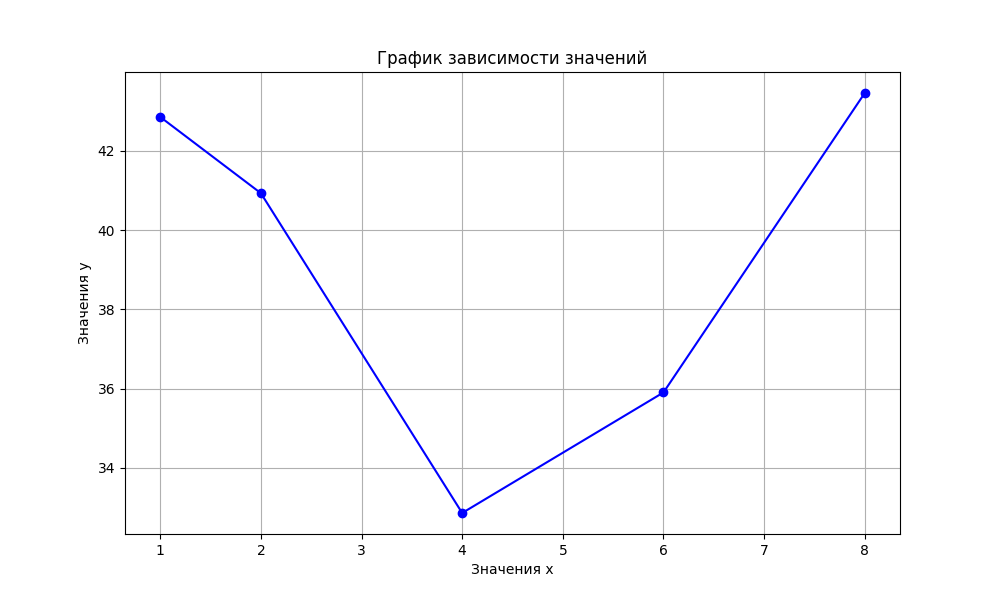
\includegraphics[width=1\linewidth]{graph.png}
    \label{fig:enter-label}
\end{figure}

\section{Заключение}

    В данной работе я изучил возможности языка C++ в работе с библиотекой MPI. 

\section{Результат запуска}
    
\begin{figure}[H]
	\centering
	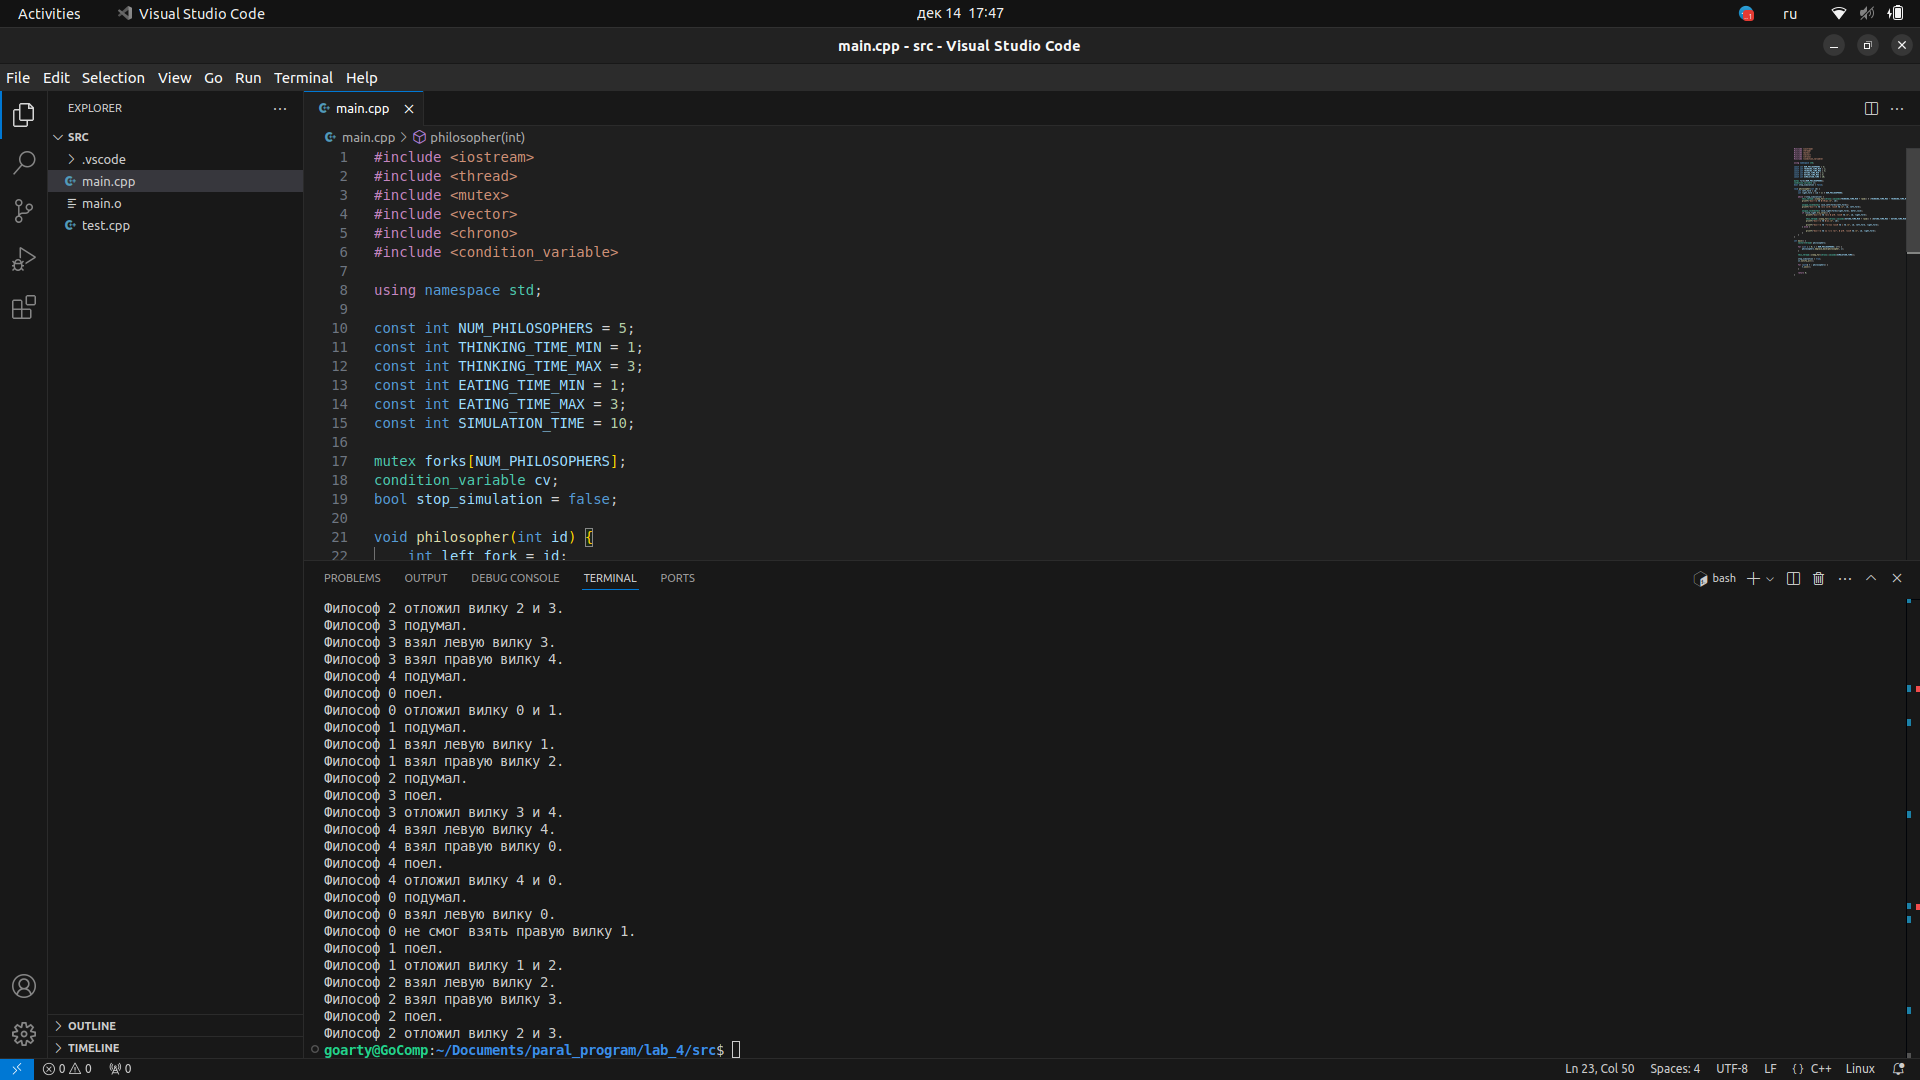
\includegraphics[width=0.8\textwidth]{picture.png}
\label{fig:picture.png}
\end{figure}

\end{document}

